\documentclass[
  % all of the below options are optional and can be left out
  % course name (default: 2IL50 Data Structures)
  course = {{ESE532 System-on-a-Chip}},
  % quartile (default: 3)
  quartile = {{}},
  % assignment number/name (default: 1)
  assignment = 1,
  % student name (default: Some One)
  name = {{Sheil Sarda}},
  % student number, NOT S-number (default: 0123456)
  studentnumber = {{}},
  % student email (default: s.one@student.tue.nl)
  email = {{sheils@seas.upenn.edu}},
  % first exercise number (default: 1)
  firstexercise = 1
]{aga-homework}
\usepackage{graphicx} 

\begin{document}


\exercise

\subexercise AWS Account ID is 540828313726.
\subexercise 
\begin{verbatim}
lscpu
Architecture:        aarch64
Byte Order:          Little Endian
CPU(s):              4
On-line CPU(s) list: 0-3
Thread(s) per core:  1
Core(s) per socket:  4
Socket(s):           1
NUMA node(s):        1
Model:               3
BogoMIPS:            166.66
L1d cache:           32K
L1i cache:           48K
L2 cache:            2048K
NUMA node0 CPU(s):   0-3
Flags:               fp asimd evtstrm aes pmull sha1 sha2 crc32 cpuid

uname -a
Linux ip-172-31-19-211.us-east-2.compute.internal 
4.14.192-147.314.amzn2.aarch64 #1 SMP Mon Aug 17 06:07:21 UTC 2020 
aarch64 aarch64 aarch64 GNU/Linux

gcc --version
gcc (GCC) 7.3.1 20180712 (Red Hat 7.3.1-9)
Copyright (C) 2017 Free Software Foundation, Inc.
This is free software; see the source for copying conditions.  There is NO
warranty; not even for MERCHANTABILITY or FITNESS FOR A PARTICULAR PURPOSE.
\end{verbatim}

\subexercise Figure of usage report from AWS:
\begin{figure}
	\centering
	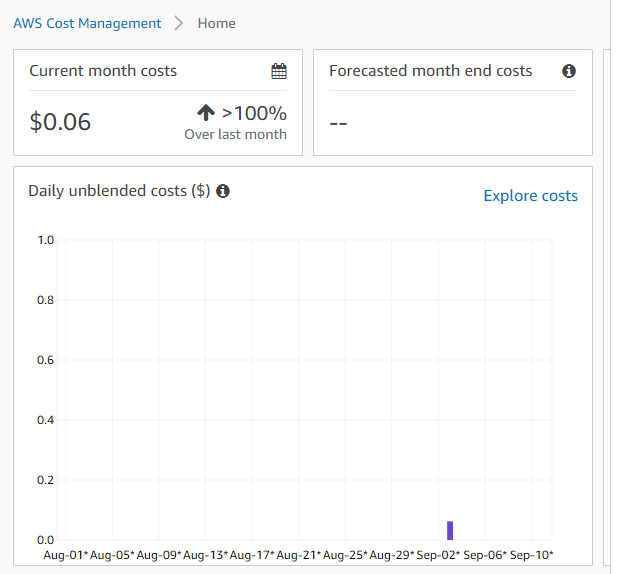
\includegraphics[width=0.7\linewidth]{figures/usage_report}
	\caption{Accurate as of 9/11/2020}
	\label{fig:usagereport}
\end{figure}

\newpage

\subexercise

\renewcommand{\theenumi}{\roman{enumi}}%
\begin{enumerate}
	\item break program.c:8
	\item clear program.c:8
	\item info locals or print
	\item step (step to the next line) or finish (step out of function)
\end{enumerate}

\exercise
\subexercise
\begin{verbatim}
[ec2-user@ip-172-31-46-28 debug_program]$ ./program                                                                 
The secret message is: Well Done!!!
\end{verbatim}

\subexercise
program.c
\begin{verbatim}
#include <stdio.h>
#include <stdlib.h>

int len(char* s) {
  int l = 0;
	
  while (*s){ 
    l++;
    s++;
  }	
  return l;
}

int rot13(int l) {
  if (l >= 'A' && l <= 'Z') l = (l - 'A' + 13) % 26 + 'A';
  if (l >= 'a' && l <= 'z') l = (l - 'a' + 13) % 26 + 'a';
  return l;
}

char* msg = "Jryy Qbar!!!\n";

int main() {
  int i = 0;
  printf("The secret message is: ");
  while (i < len(msg)) printf("%c", rot13(msg[i++]));

  return 0;
}
\end{verbatim}

Makefile
\begin{verbatim}
release:
  gcc -Wall -o program program.c
debug:
  gcc -Wall -o program program.c -g
clean:
  rm -f program
\end{verbatim}

\subexercise
Used gdb to step through the execution of the program and understand the various functions and loops. Was able to confirm my hypothesis of the len function not counting properly by observing its value staying constant through every iteration of the while loop.
\subexercise
GDB knows where functions and data are located in the executable by looking at the program's symbol table, which lists the names of variables, functions and types defined in the program. Compiling the program with -g includes the symbol table in the file.

\subexercise
Completed function: insert in order

\begin{verbatim}
// This function will perform the insertion sort and maintain the linked list
// you will need to maintain the links and properly place the new element

void insert_in_order(node_struct* new_element) {
  if(new_element == NULL){
    printf("invalid insert\n");
    return;
  }

  if(!head){
    head = new_element;   
    return;
  } 
  
  if(new_element->value < head->value){
    new_element->next = head;
    head = new_element;
  }  else  {
    node_struct* temp_head = head;
    while((temp_head->next != NULL) && (new_element->value > temp_head->next->value))
      temp_head = temp_head->next;
      
    new_element->next = temp_head->next;
    temp_head->next = new_element; 
  }
}
\end{verbatim}

Makefile
\begin{verbatim}
release:
  gcc -Wall -o program complete_function.c
debug:
  gcc -Wall -o program complete_function.c -g
clean:
  rm -f program
\end{verbatim}

\exercise

\subexercise
\begin{verbatim}
#include <stdio.h>
#include <stdlib.h>

int main()
{
  int x = 20;
  
  int *y;
  int *z;

  y = malloc(sizeof(int));
  y = 5;
  
  z = malloc(sizeof(int));
  z = 50;

  y = malloc(sizeof(int));
  y = 6;

  z = malloc(sizeof(int));
  z = 7;

  return 0;
}
\end{verbatim}

\subexercise
If program is running inside an OS, either get a stack overflow or the memory allocation via malloc() or sbrk() or mmap() will fail when you try to grow the heap. 

If program is running in a bare-metal system and if the stack grows into the heap, the C compiler will silently start to overwrite the heap's data structures. The implementation of malloc() almost certainly notices the failure and returns NULL.

\subexercise
\begin{verbatim}
#include <stdio.h>
#include <stdlib.h>

int main()
{
  int local_arr[8];
  for(int i = 0; i < 8; i++)
  {
    local_arr[i] = (8-i)*10;
  }

  int *ptr1 = &local_arr[3];
  int *ptr2 = &local_arr[7];

  // print array using ptrs
  for(int i = 7; i >= 0; i--)
  {
    printf("%d\n", *(ptr2 - i));
  }

  printf("------\n");

  int **ptr3 = &ptr2;
  for(int i = 7; i >= 0; i--)
  {
    printf("%d\n", *(*ptr3 - i));
  }
}
\end{verbatim}

\subexercise
\begin{verbatim}
#include <stdlib.h>
#include <stdio.h>

struct s2 {
  float a;
  int b;
};

struct s1 {
  int c;
  struct s2 **d;
};

int main()
{
  struct s1 x[5];
  int b_addr = &((*(x->d))->b);

  printf("Address of b: %x\n", b_addr);
}
\end{verbatim}

\subexercise
\begin{verbatim}
#include <stdio.h>
#include <stdlib.h>

int main()
{
  double a[] = {3.14, 2.71};

  unsigned char *to_print = (unsigned char*)a;
  for (int i = 0; i < 8; ++i)
  {	
    printf("%x\n", *to_print);
    to_print = to_print + sizeof(char);
  }
}
\end{verbatim}

\subexercise
\begin{verbatim}
#include <stdio.h>
#include <stdlib.h>

void temp(int i) {
  int a[2];
  int b[3];
  int *c;
  int *d;
  c = (int *)malloc(sizeof(int) * 4);
  d = (int *)malloc(sizeof(int) * 5);

  // print addresses for arrays here....
  printf("Address for a-d:\n");
  printf("%x\n", &a[0]);
  printf("%x\n", &b[0]);

  printf("%x\n", c);
  printf("%x\n", d);

  return;
}

int main() {
  temp(1);
  return 0;
}
\end{verbatim}

\subexercise
\begin{verbatim}
int a[3];
int b[4];
int c[5];

// intervening code omitted

b[4]=13;
\end{verbatim}
What might happen with the following code? Many different things could happen. Give multiple answers. For each identified case, what happens and why (2 lines max for each case).

\renewcommand{\theenumi}{Case \Roman{enumi}}%
\begin{enumerate}
	\item Assuming both b and c are allocated in contiguous blocks of the stack. In this case, assigning 13 to one element beyond b will overwrite the first element of c. 
	\item Assuming b and c are not allocated in contiguous blocks of the stack, the behavior of overwriting a piece of memory which is beyond the range that b spans is undefined. It might lead to errors further down in the execution of the program when the overwritten block is accessed again.
\end{enumerate}




\subexercise
Code:
\begin{verbatim}
#include "stdio.h"
#include "stdlib.h"

int main(int argc, char** argv) {
  unsigned char a[3] = {0xFF, 0x01, 73};
  unsigned char sum;
  unsigned int intsum;
 
  signed char sa[3] = {127, 1, 33};
  signed char ssum;
  signed int sintsum;

  fprintf(stdout, "Unsigned:\n");
  for (int i = 0; i < 3; i++)
    for (int j = 0; j < 3; j++) {
      sum = a[i] + a[j];
      intsum = a[i] + a[j];
      fprintf(stdout, "in decimal: %d+%d=%d (intsum=%d)\t", a[i], a[j], sum, 
      intsum);
      fprintf(stdout, "in hexadecimal: %x+%x=%x (intsum=%x)\n", a[i], a[j], sum, 
      intsum);
    }

  fprintf(stdout, "Signed:\n");
  for (int i = 0; i < 3; i++)
    for (int j = 0; j < 3; j++) {
      ssum = sa[i] + sa[j];
      sintsum = sa[i] + sa[j];
      fprintf(stdout, "in decimal: %d+%d=%d (intsum=%d)\t", sa[i], sa[j], 
      ssum, sintsum);
      fprintf(stdout, "in hexadecimal: %x+%x=%x (intsum=%x)\n", sa[i], sa[j], 
      ssum, sintsum);
    }
}
\end{verbatim}

Results:
\begin{verbatim}
[ec2-user@ip-172-31-46-28 c-tutorial]$ ./explain
Unsigned:
in decimal: 255+255=254 (intsum=510)    in hexadecimal: ff+ff=fe (intsum=1fe)
in decimal: 255+1=0 (intsum=256)        in hexadecimal: ff+1=0 (intsum=100)
in decimal: 255+73=72 (intsum=328)      in hexadecimal: ff+49=48 (intsum=148)
in decimal: 1+255=0 (intsum=256)        in hexadecimal: 1+ff=0 (intsum=100)
in decimal: 1+1=2 (intsum=2)            in hexadecimal: 1+1=2 (intsum=2)
in decimal: 1+73=74 (intsum=74)         in hexadecimal: 1+49=4a (intsum=4a)
in decimal: 73+255=72 (intsum=328)      in hexadecimal: 49+ff=48 (intsum=148)
in decimal: 73+1=74 (intsum=74)         in hexadecimal: 49+1=4a (intsum=4a)
in decimal: 73+73=146 (intsum=146)      in hexadecimal: 49+49=92 (intsum=92)
Signed:
in decimal: 127+127=-2 (intsum=254)     in hexadecimal: 7f+7f=fffffffe (intsum=fe)
in decimal: 127+1=-128 (intsum=128)     in hexadecimal: 7f+1=ffffff80 (intsum=80)
in decimal: 127+33=-96 (intsum=160)     in hexadecimal: 7f+21=ffffffa0 (intsum=a0)
in decimal: 1+127=-128 (intsum=128)     in hexadecimal: 1+7f=ffffff80 (intsum=80)
in decimal: 1+1=2 (intsum=2)            in hexadecimal: 1+1=2 (intsum=2)
in decimal: 1+33=34 (intsum=34)         in hexadecimal: 1+21=22 (intsum=22)
in decimal: 33+127=-96 (intsum=160)     in hexadecimal: 21+7f=ffffffa0 (intsum=a0)
in decimal: 33+1=34 (intsum=34)         in hexadecimal: 21+1=22 (intsum=22)
in decimal: 33+33=66 (intsum=66)        in hexadecimal: 21+21=42 (intsum=42)
\end{verbatim}
Explanation of results:
Difference between unsigned char and integer sums is that the range of an unsigned char is 0 (0x00) to 255 (0xff). When the char variable overflows, the C compiler creates a wraparound effect where the char gets reset to 0 again. To illustrate, 255 + 1 = 1 + 255 = 0. On the other hand, the unsigned int variable has a range of 0x00000000 to 0xffffffff so no overflow or wraparound occurs.

\paragraph{}
Difference between char and integer sums is that the range of a char is -128 (0xff) to 127 (0x7f). Similar to the above explanation, when an overflow occurs, the C compiler resets the char to -127 and wraps around. To illustrate, 1 + 127 = 127 + 1 = -128. On the other hand, the signed int variable has a much larger range so no overflow or wraparound occurs.

\subexercise
Purpose of the preprocessor: the C preprocessor expands macros and include statements and passes the result to the actual compiler. It replaces short cuts with more code, so the output of this stage is just C code.

\paragraph{}
Purpose of the compiler: the compiler translates preprocessed C code into assembly code, performing various optimizations along the way as well as register allocation. A compiler generates assembly code specific to a particular architecture.

\paragraph{}
It is the job of the linker to use the notes provided by the assembler about the memory layout and assign absolute memory locations, as well as resolve any references. The linker produces a binary executable that can be run from the command interface.

\subexercise
\renewcommand{\theenumi}{\roman{enumi}}%
\begin{enumerate}
	\item Double check the path of the header file that the preprocessor is unable to find.

	\item 	Add additional directories to the search path using -Idir, which causes dir to be searched after the current directory (for the quote form of the directive) and ahead of the standard system directories. 
	
	\item	If you need separate control over the search paths for the quote and angle-bracket forms of the ‘\#include’ directive, you can use the -iquote and/or -isystem options instead of -I. 	

\end{enumerate}

\subexercise
\renewcommand{\theenumi}{\roman{enumi}}%
\begin{enumerate}
	\item  Linker finds a declaration of a function but no definition of it. This occurs when the compiler is provided with the function header, but there was no such function defined anywhere, so the compilation stage passes but the linker exits with an Undefined reference error. To fix this error, we need to add a definition for the function.
	
	\item An alternative situation arises where the source for the function is in a separate file but both source files are not linked. Here the fix is to link both the source files.
	
	\item Another common error is to provide a definition that does not match up with declaration (or vice versa). For example, if we provide a definition of the function whose signatures (name, plus parameter list types) doesn't match the declaration. so the definition actually defines a completely different function from the one in the declaration. 
	
\end{enumerate}


\end{document}
